%%%%%%%%%%%%%%%%%%%%%%%%%%%%%%%%%%%%%%%%%
% Beamer Presentation
% LaTeX Template
% Version 1.0 (10/11/12)
%
% This template has been downloaded from:
% http://www.LaTeXTemplates.com
%
% License:
% CC BY-NC-SA 3.0 (http://creativecommons.org/licenses/by-nc-sa/3.0/)
%
%%%%%%%%%%%%%%%%%%%%%%%%%%%%%%%%%%%%%%%%%

%----------------------------------------------------------------------------------------
%	PACKAGES AND THEMES
%----------------------------------------------------------------------------------------

\documentclass{beamer}

\mode<presentation> {

% The Beamer class comes with a number of default slide themes
% which change the colors and layouts of slides. Below this is a list
% of all the themes, uncomment each in turn to see what they look like.

%\usetheme{default}
%\usetheme{AnnArbor}
%\usetheme{Antibes}
%\usetheme{Bergen}
%\usetheme{Berkeley}
%\usetheme{Berlin}
%\usetheme{Boadilla}
%\usetheme{CambridgeUS}
%\usetheme{Copenhagen}
%\usetheme{Darmstadt}
%\usetheme{Dresden}
%\usetheme{Frankfurt}
%\usetheme{Goettingen}
%\usetheme{Hannover}
%\usetheme{Ilmenau}
%\usetheme{JuanLesPins}
%\usetheme{Luebeck}
%\usetheme{Madrid}
%\usetheme{Malmoe}
%\usetheme{Marburg}
%\usetheme{Montpellier}
%\usetheme{PaloAlto}
%\usetheme{Pittsburgh}
%\usetheme{Rochester}
%\usetheme{Singapore}
%\usetheme{Szeged}
%\usetheme{Warsaw}

% As well as themes, the Beamer class has a number of color themes
% for any slide theme. Uncomment each of these in turn to see how it
% changes the colors of your current slide theme.

%\usecolortheme{albatross}
%\usecolortheme{beaver}
%\usecolortheme{beetle}
%\usecolortheme{crane}
%\usecolortheme{dolphin}
%\usecolortheme{dove}
%\usecolortheme{fly}
%\usecolortheme{lily}
%\usecolortheme{orchid}
%\usecolortheme{rose}
%\usecolortheme{seagull}
%\usecolortheme{seahorse}
%\usecolortheme{whale}
%\usecolortheme{wolverine}

%\setbeamertemplate{footline} % To remove the footer line in all slides uncomment this line
%\setbeamertemplate{footline}[page number] % To replace the footer line in all slides with a simple slide count uncomment this line

%\setbeamertemplate{navigation symbols}{} % To remove the navigation symbols from the bottom of all slides uncomment this line
}
\usepackage[utf8]{inputenc}
\usepackage[T1]{fontenc}
\usepackage{parskip}
\usepackage{amsmath}
\usepackage{graphicx}
\usepackage{media9}
\usepackage[utf8]{inputenc} % allow utf-8 input
\usepackage[T1]{fontenc}    % use 8-bit T1 fonts
\usepackage{hyperref}       % hyperlinks
\usepackage{url}            % simple URL typesetting
\usepackage{booktabs}       % professional-quality tables
\usepackage{amsfonts}       % blackboard math symbols
\usepackage{nicefrac}       % compact symbols for 1/2, etc.
\usepackage{microtype}      % microtypography
\usepackage{times}
\usepackage{multimedia}
\newtheorem{thm}{Theorem}

%\usepackage{hyperref}
%\usepackage{algorithm}
%\usepackage{algpseudocode}
%\usepackage{algorithmicx}
\usepackage{amsthm,amsmath,amssymb,natbib,amsfonts,graphicx,epsfig,pgf,subfig,rotating,longtable,booktabs, colortbl, graphics,fontenc}
%\usepackage[linesnumbered, ruled, vlined]{algorithm2e}
%\usepackage[options ]{algorithm2e}
\usepackage{algorithm}
\usepackage{algorithmic}
\usepackage{tabularx}
\usepackage{wrapfig}
\newcommand{\argmax}{\operatornamewithlimits{argmax}}


	% drawing the background after the foreground



	% drawing the background after the foreground



% Table float box with bottom caption, box width adjusted to content

\long\def\/*#1*/{}
%----------------------------------------------------------------------------------------
%	TITLE PAGE
%----------------------------------------------------------------------------------------


\title[]{Neural Autoregressive Flows} % The short title appears at the bottom of every slide, the full title is only,on the title page

\author[]{Chin-Wei Huang, David Krueger, Alexandre Lacoste, Aaron Courville \\[1cm]Presented by\\[.8em]{\large Avideep Mukherjee}\\Advised by\\{\large Prof. Vinay P. Namboodiri} \\[1em] {\footnotesize Department of Computer Science and Engineering\\ Indian Institute of Technology Kanpur}} % Your name
\institute[] % Your institution as it will appear on the bottom of every slide, may be shorthand to save space

\date{\today} % Date, can be changed to a custom date

\begin{document}

\begin{frame}
\titlepage % Print the title page as the first slide
\end{frame}

\begin{frame}{Outline}
    \begin{itemize}
        \item Types of Generative Models
        \item Normalizing Flows
        \item Autoregressive Models
        \item Inverse Autoregressive Flow
        \item Neural Autoregressive Flow
    \end{itemize}
\end{frame}
\begin{frame}
\frametitle{Types of Generative Models} % Table of contents slide, comment this block out to remove it
% Throughout your presentation, if you choose to use \section{} and \subsection{} commands, these will automatically be printed on this slide as an overview of your presentation
 
\begin{figure}[h]
    \centering
    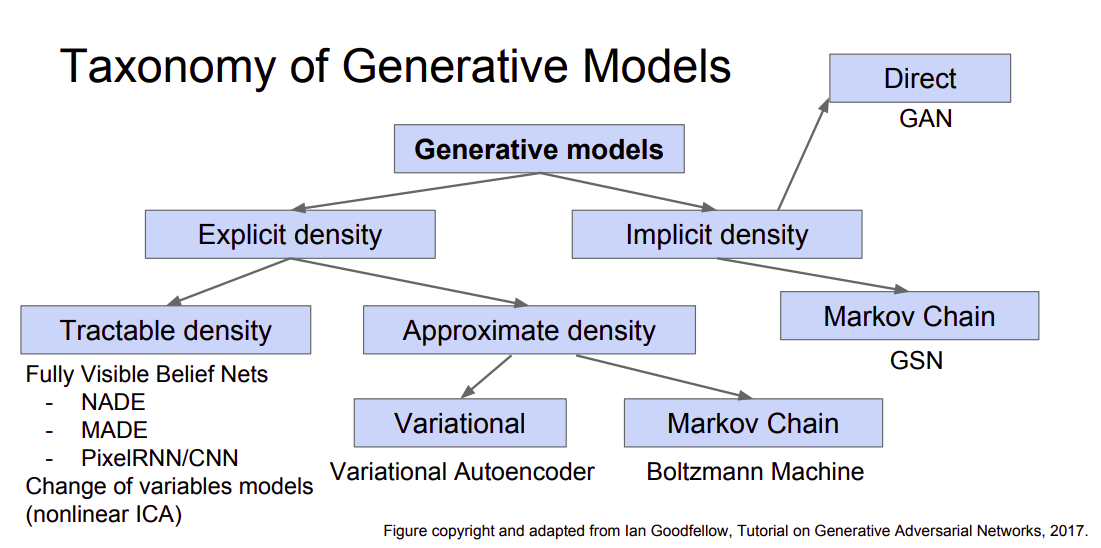
\includegraphics[width=\textwidth,keepaspectratio]{generative-models.png}
    \label{fig:my_label}
\end{figure}




\end{frame}


\begin{frame}

\frametitle{Normalizing Flows}
\begin{itemize}
    \item Transform an \textit{‘easy' paramaterizable base distribution} in a \textit{more complex approximation} for the posterior distribution (\cite{rezende2015variational}).
    \pause
    \item Pass the base distribution through a series (flow) of transformations (\textit{invertible, bijective mappings}).
    \pause
    \item $\mathbf{z} \in \mathbb{R}^d$ and $\mathbf{y} = f(\mathbf{z})$ where $f: \mathbb{R}^d \mapsto \mathbb{R}^d$  Let $\mathbf{z} \sim q(\mathbf{z})$. According to change of variable formula :
\end{itemize}
\pause
\begin{equation}
    q_y(\mathbf{y}) = q(\mathbf{z}) \left|
    \mathrm{det} \frac{
      \partial f^{-1}
    }{
      \partial \mathbf{z}\
    }
  \right|
  = q(\mathbf{z}) \left|
    \mathrm{det} \frac{
      \partial f
    }{
      \partial \mathbf{z}\
    }
  \right| ^{-1}
\end{equation}
\end{frame}

\begin{frame}{Normalizing Flows}
Apply a series of such mappings $f_k$, $k \in {1,\dots, K}$ with $K \in \mathbb{N}_+$ and obtain a \textbf{normalizing flow}.
\pause
\begin{equation}
    \mathbf{x} = \mathbf{z}_K = f_K \circ \dots \circ f_1 (\mathbf{z}_0), \quad \mathbf{z}_0 \sim q_0(\mathbf{z}_0)
\end{equation}
\pause
\begin{equation}
    \mathbf{z}_K \sim q_K(\mathbf{z}_K) = q_0(\mathbf{z}_0) \prod_{k=1}^K
  \left|
    \mathrm{det} \frac{
      \partial f_k
    }{
      \partial \mathbf{z}_{k-1}\
    }
  \right| ^{-1}
\end{equation}
\pause
\begin{equation}
    \log q(\mathbf{z}_K) = \log q(\mathbf{z}_0) - \sum_{k=1}^{K} \log
    \left| \mathrm{det} \frac{\partial{f_k}}{\partial{\mathbf{z}_{k-1}}}
    \right|
\end{equation}
\end{frame}


\begin{frame}{Normalizing Flows}
Loss Function :\footnote{For the derivation of the Variational Free Energy, see Slide \ref{appendix}: Appendix}
\begin{eqnarray}
\mathcal{F}(x) &=& E_{\mathbf{z} \sim q}[\log q(\mathbf{z}) - \log P(x, \mathbf{z})] \\
&=&  E_{z \sim q}[\log q(\mathbf{z_K}) - \log P(x, \mathbf{z_K})] \\
&=&  E_{z \sim q}[\log q(\mathbf{z_0}) - \sum_{k=1}^{K} \log \left| \det \frac{\partial{f_k}}{\partial{\mathbf{z_{k-1}}}} \right| - \log P(x, \mathbf{z_K})] \label{vfeflow}
\end{eqnarray}
\end{frame}
\begin{frame}{Planar Flows}
   \begin{itemize}
       \item Transformation function $f_k$ should satisfy two properties:
       \begin{itemize}
           \item It is easily invertible.
           \item Its Jacobian determinant is easy to compute.
       \end{itemize}
       \item Planar Flows : $f(\mathbf{z}) = \mathbf{z} + \mathbf{u} h(\mathbf{w}^T \mathbf{z} + b)$ 
   \begin{eqnarray}
    \psi(z) &=& h'(w^Tz + b)w \\
    \left| \det \frac{\partial{f}}{\partial{z}} \right| &=& \left| \det(I + u \psi (z)^T)  \right| = \left| 1+u^T \psi (z)  \right|
    \end{eqnarray}
    \item Matrix-determinant lemma : $\det(I + uv^T) = (1 + v^Tu)$
    \end{itemize}
\end{frame}
\begin{frame}{Normalizing Flows}
    \begin{figure}
        \centering
        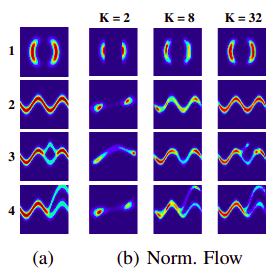
\includegraphics[width=60mm,scale=0.65]{nf-result.png}
        \caption{(a) Target Distribution. (b) ) Approx posterior using NF\footnote{Image Source : \cite{rezende2015variational}}}
        \label{fig:my_label}
    \end{figure}
\end{frame}
\begin{frame}{Autoregressive Models}
    \begin{itemize}
        \item Autoregressive constraint : each output only depends on the data observed in the past, but not on the future ones. 
        \pause
        \begin{equation}
            p(\mathbf{x}) = \prod_{i=1}^{D} p(x_i\vert x_1, \dots, x_{i-1}) = \prod_{i=1}^{D} p(x_i\vert x_{1:i-1})
        \end{equation}
    \end{itemize}
\end{frame}
\begin{frame}{Autoregressive Models}

\begin{figure}
    \centering
    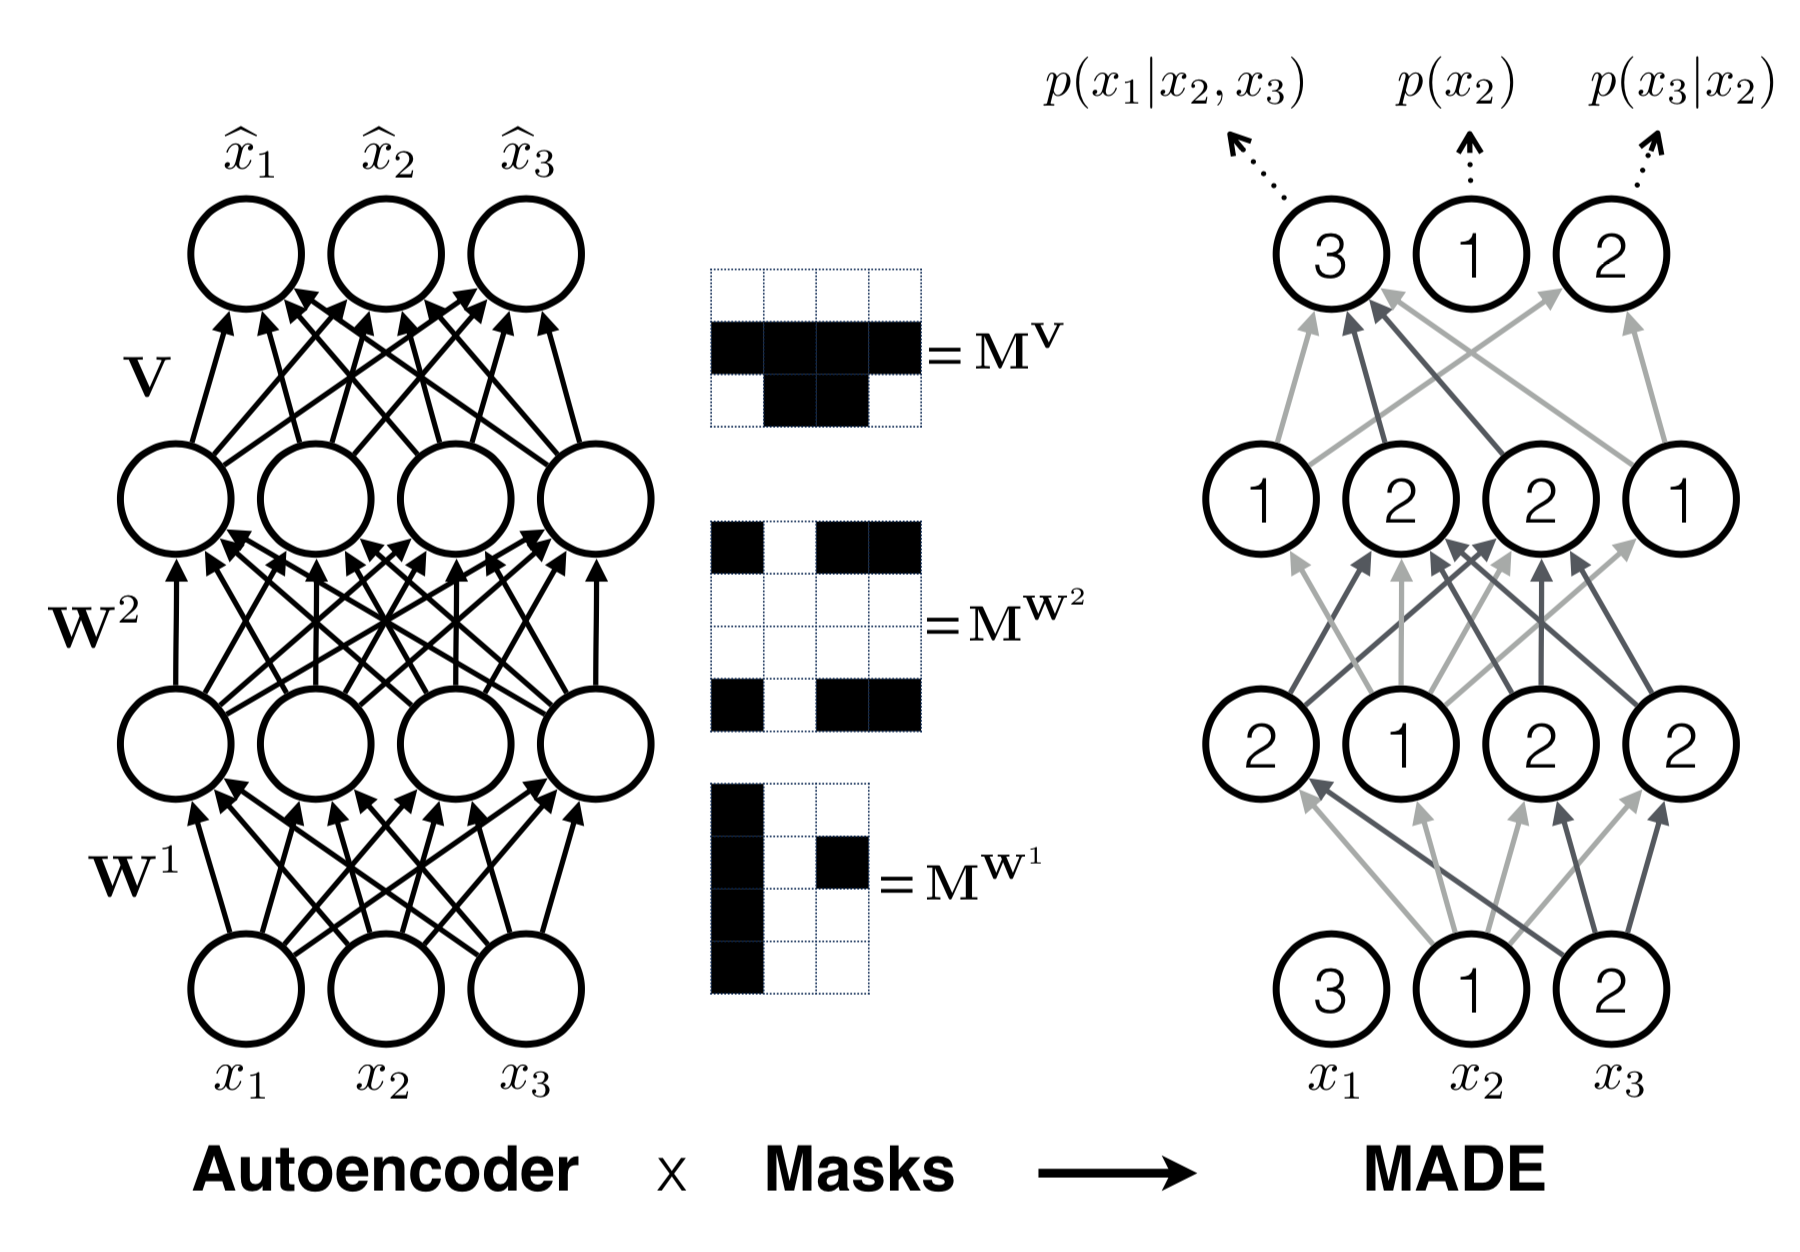
\includegraphics[width=100mm, scale=0.7]{MADE.png}
    \caption{Demonstration MADE in a 3-layer NN. \cite{germain2015made}\footnote{Image Source : \cite{germain2015made}}}
    \label{fig:made}
\end{figure}
    
\end{frame}
\begin{frame}{Autoregressive Flows}
\begin{itemize}
    \item flow transformation framed as an autoregressive model — \textbf{autoregressive flow}.
    \pause
    \item Autoregressive functions do have tractable determinant Jacobians.
    \pause
    \item Let $f(\mathbf{z}) = \mathbf{z'}$. An autoregressive function would look like this: 
    \begin{eqnarray}
        z’_i = f(z_{1:i}) \quad \forall i
    \end{eqnarray}
    \pause
    \item The Jacobian $J = \frac{\partial{z’}}{\partial{z}}$ becomes lower triangular.
    \begin{eqnarray}
        \det J = \prod_{i=1}^D J_{ii}
    \end{eqnarray}
\end{itemize}
\end{frame}
\begin{frame}{Autoregressive Transformation}
\begin{itemize}
    \item Let $z’ = f(z)$, and the first dimension of the transformed variable be defined by:
    \begin{eqnarray}
    z &\sim& \mathcal{N}(0, I) \quad [\text{base distribution: } q(\mathbf{z})] \\
    z’_0 &=& \mu_0 + \sigma_0 \odot z_0 \quad [\text{Randomly Sampled}]  \label{first_step}
    \end{eqnarray}
    \pause
    \item The other dimensions $i>0$ are computed by :
\end{itemize}
\begin{eqnarray}
z'_i = \mu_i(z'_{1:i-1}) + \sigma_i(z'_{1:i-1}) \cdot z_i \label{nth_step}
\end{eqnarray}
    
\end{frame}
\begin{frame}{Inverse Autoregressive Transformation}
\begin{itemize}
    \item Inverse of Equation  (\ref{first_step}) and (\ref{nth_step}) are :
    \begin{eqnarray}
    z_0 &=& \frac{z'_0 - \mu_0}{\sigma_0} \label{iart0} \\
    z_i &=& \frac{z'_i - \mu(z'_{1:i-1}) }{\sigma(z'_{1:i-1})} \label{iart}
    \end{eqnarray}
    \pause
    \item $\mu(\cdot)$ and $\sigma(\cdot)$ are independent on $z'_i$, $\therefore$ we have a tractable determinant Jacobian
    \pause
    \begin{eqnarray}
    \det \left| \frac{d{\bf z}}{d{\bf z'}} \right| &=& \prod_{i=1}^D  \frac{1}{\sigma_i(z_{1:i-1})} \\
    \log \det \left| \frac{d{\bf z}}{d{\bf z'}} \right| &=& \sum_{i=1}^D - \log \sigma_i(z_{1:i-1})
    \end{eqnarray}
\end{itemize}
\end{frame}
\begin{frame}{Inverse Autoregressive Flow (IAF)}
\begin{itemize}
    \item \cite{kingma2016improved} has defined two functions ${\bf s}_t = \frac{1}{\sigma_t(\cdot)}$ and ${\bf m}_t = \frac{-\mu_t(\cdot)}{\sigma_t(\cdot)}$.
    \item ${\bf s}_t$ and ${\bf m}_t$ can be modeled by \textbf{autoregressive neural networks}.
\end{itemize}
\begin{eqnarray}
z_t &=& \frac{z_{t-1} - \mu_t(z_{t-1}) }{\sigma_t(z_{t-1})} \\
    &=& \frac{z_{t-1}}{\sigma_t(z_{t-1})} - \frac{\mu_t(z_{t-1})) }{\sigma_t(z_{t-1}) } \\
    &=& z_{t-1} \odot {\bf s}_t(z_{t-1})  + {\bf m}_t (z_{t-1}) \label{upd}
\end{eqnarray}
\pause
\begin{itemize}
    \item And finally for numerical stability they modify Equation (\ref{upd})
\end{itemize}
\begin{eqnarray}
g_t &=& \text{sigmoid}({\bf s}_t(z_{t-1}))  \\
z_t &=& z_{t-1} \odot g_t  + (1 - g_t) \odot {\bf m}_t (z_{t-1}) \label{transf}
\end{eqnarray}
\end{frame}
\begin{frame}{Neural Autoregressive Flow}
\begin{itemize}
    \item Re-write Equation (\ref{transf}) as a combination of an autoregressive \textbf{conditioner}, $c$ and an invertible \textbf{transformer}, $\tau$
\end{itemize}
\begin{eqnarray}
y \doteq f(x_{1:t}) = \tau(c(x_{1:t-1}),x_t)
\end{eqnarray}
\pause
\begin{itemize}
    \item $c$ can be computed by an autoregressive model such as \textbf{MADE}(\cite{germain2015made}). 
    \pause
    \item The transformation function, $\tau$ as given by \cite{kingma2016improved} is:
\end{itemize}
\begin{eqnarray}
\tau(\mu, \sigma, x_t) = \sigma x_t + (1-\sigma)\mu \label{aaf}
\end{eqnarray}
\pause
Notice the similarity between Eq (\ref{transf}) and (\ref{aaf}).
\end{frame}
\begin{frame}{Neural Autoregressive Flow}
    \begin{itemize}
        \item Two requirements for transformer $\tau$
        \begin{itemize}
            \item must be invertible as a function of $x_t$
            \item $\frac{dy_t}{dx_t}$ must be cheap to compute.
        \end{itemize}
        \item In IAF, $\tau$ is affine, trivially invertible. In NAF, $\tau$ is a neural network.
        \begin{equation}
            \tau(c(x_{1:t-1}),x_t) = DNN(x_t; \phi = c(x_{1:t-1}))
        \end{equation}
        \item where $\phi$ are the \textbf{pseudo-parameters}
    \end{itemize}
\end{frame}
\begin{frame}{Architecture of NAF}
\begin{figure}
    \centering
    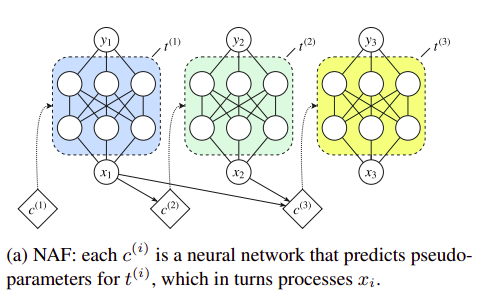
\includegraphics[width=100mm,scale=0.7]{naf.png}
    \caption{Block Diagram of NAF Architecture.Here $t^{(i)}$ means $\tau^{(i)}$\footnote{Image Source : \cite{de2019block}}}
    \label{fig:naf}
\end{figure}
\end{frame}
\begin{frame}{Architecture of NAF}
\begin{figure}
    \centering
    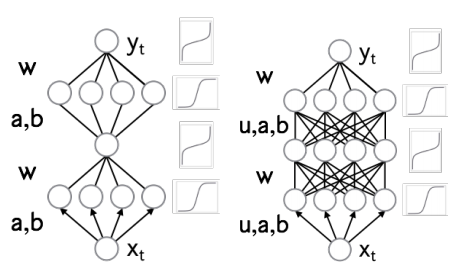
\includegraphics[width=100mm,scale=0.7]{dsf-ddsf.png}
    \caption{Proposed Transformer Networks ($\tau$). \textbf{Left}: Deep Sigmoidal Flows(DSF). \textbf{Right}: Deep Dense Sigmoidal Flows(DDSF).\footnote{Image Source: \cite{huang2018neural}}}
    \label{fig:dsf-ddsf}
\end{figure}
\end{frame}
\begin{frame}{More on DSF and DDSF}
\begin{itemize}
    \item DSF:
    \begin{equation}
        y_t = \sigma^{-1}(\underbrace{w^T}_{1 \times d}\cdot \sigma(\underbrace{a}_{d\times 1}\cdot\underbrace{x_t}_{1\times 1}+\underbrace{b}_{d\times 1}))
    \end{equation}
    where $0 < w_{i,h} < 1, \sum_i w_{i,j} = 1$ and $d$ denotes the number of hidden units.\
    \pause
    \item DDSF : 
    \begin{equation}
        h^{(l+1)} = \sigma^{-1}(\underbrace{w^{(l+1)}}_{d_{l+1}\times d_{l+1}}\cdot \sigma(\underbrace{a^{(l+1)}}_{d_{l+1}}\odot\underbrace{u^{(l+1)}}_{d_{l+1}\times d_l}\cdot\underbrace{h^{(l)}}_{d_l}+\underbrace{b^{(l+1)}}_{d_{l+1}}))
    \end{equation}
    for $1 < l < L$, $h_0 = x$ and $y = h_L$;$d_0 = d_L = 1$; $\mathbf{w}$ and $\mathbf{u}$ are softmax-weighted.
\end{itemize}
    
\end{frame}
\begin{frame}{Result}
\begin{figure}
    \centering
    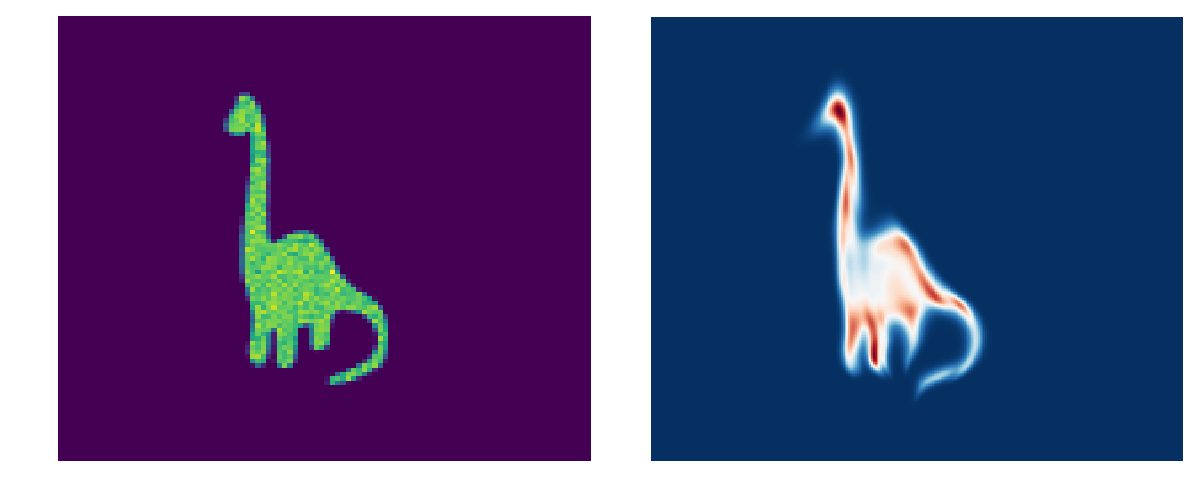
\includegraphics[width = \textwidth, \keepaspectratio]{naf-result-dino.png}
    \caption{\textbf{Left}: Target Distribution, \textbf{Right}: Modeled by NAF.\footnote{Image Source: https://medium.com/element-ai-research-lab/neural-autoregressive-flows-f164d6b8e462 }\\Any resemblance of the distribution with any animal, living or extinct, is purely co-incidental.}
    \label{fig:my_label}
\end{figure}
\end{frame}
\begin{frame}{Comparison with AAF(IAF)}
\begin{figure}
    \centering
    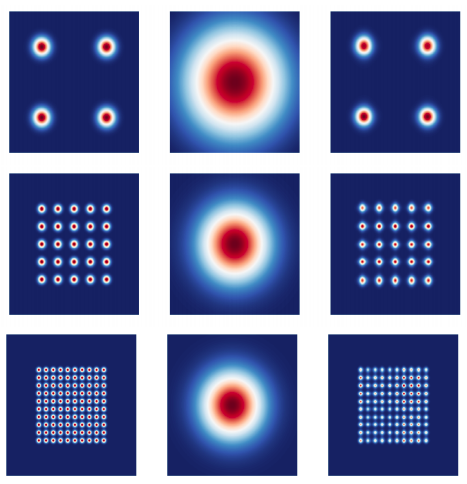
\includegraphics[width=50mm,scale=0.5]{naf-result.png}
    \caption{Fitting grid of Gaussian distributions using maximum
likelihood. Left: true distribution. Center: AAF. Right: NAF\footnote{Image Source : \cite{huang2018neural}}}
    \label{fig:naf-result}
\end{figure}
\end{frame}

\begin{frame}{Detailed Comparison}
\begin{figure}
    \centering
    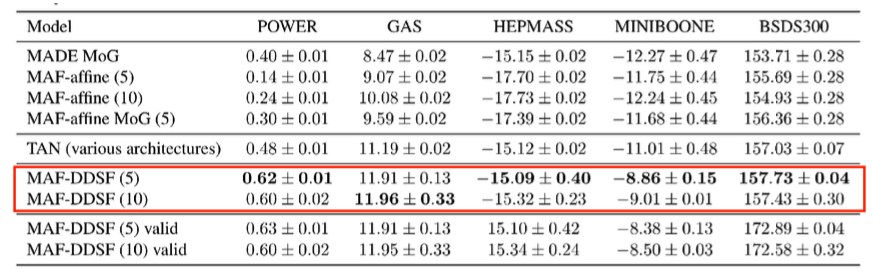
\includegraphics[width=110mm]{naf-table.png}
    \caption{Test log-likelihood and error bars of 2 standard deviations on the 5 datasets.\footnote{Table taken from : https://medium.com/element-ai-research-lab/neural-autoregressive-flows-f164d6b8e462}}
    \label{fig:my_label}
\end{figure}
    
\end{frame}
\begin{frame}[allowframebreaks]
\frametitle{References}
\bibliography{main.bib}
\bibliographystyle{apalike}

\end{frame}
\begin{frame}{Acknowledgements}
    Slides made with help from the following blogs :
    \begin{itemize}
        \item https://lilianweng.github.io/lil-log/2018/10/13/flow-based-deep-generative-models.html
        \item http://akosiorek.github.io/ml/2018/04/03/norm\_flows.html
        \item https://medium.com/element-ai-research-lab/neural-autoregressive-flows-f164d6b8e462
        \item https://www.ritchievink.com/
    \end{itemize}
\end{frame}

\begin{frame}{}
  \centering \LARGE
  \emph{Thank you}
\end{frame}
\begin{frame}{Appendix}
\label{appendix}
    \begin{itemize}
        \item Derivation of the variational free enery :
    \end{itemize}
    \begin{eqnarray}
    F(x) &=& D_{KL}(Q(z) || P(z)) - E_{z \sim Q}[\log P(x|z)]\\
    &=& \int_{z} Q(z) \log \frac{Q(z)}{P(z)} dz - E_{z \sim Q}[\log P(x|z)]\\
    &=& E_{z \sim Q}[\log \frac{Q(z)}{P(z)}] - E_{z \sim Q}[\log P(x|z)]\\
    &=& E_{z \sim Q}[\log \frac{Q(z)}{P(z)} - \log P(x|z)]  \\
    &=& E_{z \sim Q}[\log Q(z) - \log P(z)  - \log P(x|z)]  \\
    &=& E_{z \sim Q}[\log Q(z) - (\log P(z)  + \log P(x|z))]\\
    &=& E_{z \sim Q}[\log Q(z) - \log P(x, z))]
    \end{eqnarray}
\end{frame}
\end{document} 